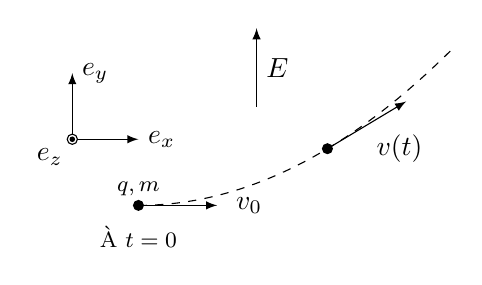
\begin{tikzpicture}
\shorthandoff{:}
%%%%%%%%%%% repère
\begin{scope}[scale=0.84,shift = {(-1,1)}]
\draw[-latex] (0,0) -- +(1,0) node[right]{$\vv{e_x}$};
\draw[-latex] (0,0) -- +(0,1) node[right]{$\vv{e_y}$};
\filldraw[fill=white,draw=black] circle(2.2pt) node[below left]{$\vv{e_z}$};
\fill[] (0,0) circle(1.2pt);
\end{scope}

%%%%%%%%%%%%%%%%%%%%%%
\draw[-latex] (1.5,1.25) -- +(0,1) node[midway,right]{$\vv{E}$};
\draw[smooth,samples=200,dashed,domain=0:4] plot (\x,\x/8*\x);
\fill (0,0) circle(2pt) node[above]{\footnotesize $q,m$};
\draw[-latex] (0,0) -- +(1,0) node[right]{~$\vv{v_0}$};
\draw (0,-0.4) node[]{\footnotesize \`A $t=0$};

\fill (2.4,0.72) circle(2pt);
\draw[-latex] (2.4,0.72) -- +(1,0.6) node[midway,below right]{$\vv{v}(t)$};
\end{tikzpicture}

